\documentclass[conference]{IEEEtran}
\IEEEoverridecommandlockouts
% The preceding line is only needed to identify funding in the first footnote. If that is unneeded, please comment it out.
\usepackage{cite}
\usepackage{amsmath,amssymb,amsfonts}
\usepackage{algorithmic}
\usepackage{graphicx}
\usepackage{textcomp}
\usepackage{xcolor}
\def\BibTeX{{\rm B\kern-.05em{\sc i\kern-.025em b}\kern-.08em
    T\kern-.1667em\lower.7ex\hbox{E}\kern-.125emX}}
\begin{document}
\title{Security-Aware Clock Tree Synthesis through Weighted Data-Arrival Alignment}
\author{\IEEEauthorblockN{Kairav Kumar}
\IEEEauthorblockA{\textit{Bachelor Thesis Project}\\Under the supervision of Prof. Chandan Karfa}}
% Supply verified institution, department and email before submission.
\maketitle
\begin{abstract}
Masking protects cryptographic computations by distributing
sensitive values across randomized shares, but its physical
implementation must also account for transient switching and
signal-arrival differences. Minimizing clock skew alone does
not control the relative arrival of secret-dependent signals
at combinational gates. This motivates incorporating
security-relevant data-arrival relationships into clock-tree
synthesis.

This paper presents a security-aware clock-tree synthesis
framework that coordinates register clock arrivals to improve
signal alignment at structurally identified sensitive gates.
The framework uses secret and share provenance to prioritize
reconvergent logic and preserves individual launch-source
contributions during static timing analysis. A linear-programming
formulation determines requested clock arrivals subject to
timing constraints. A cost-aware asymmetric constructor then
realizes these requests through shared clock branches. Its
bounded dynamic-programming search retains alternative subtree
implementations and buffer strengths, balancing arrival accuracy
against estimated implementation cost. The approach preserves
the masked datapath, register placement, and pipeline structure.

The clock-tree constructor operates on timing targets and
physical sink information, while secret-share annotations
provide circuit-specific security priorities. Evaluation on a masked PRESENT
substitution layer demonstrates improved data-arrival
alignment at marked sensitive gates and reduced aggregate
modeled glitching power, while maintaining comparable total
power and cell area. These results support incorporating
security-relevant timing objectives into clock-tree synthesis
as a practical complement to hardware masking.
\end{abstract}
\begin{IEEEkeywords}
clock tree synthesis, masked hardware, data skew, linear programming, dynamic programming, side-channel evaluation
\end{IEEEkeywords}
\section{Introduction}
Physical timing influences when internal signals change, even when two implementations compute the same Boolean function. If inputs of a combinational gate settle at different times, intermediate combinations can produce additional output transitions. In a masked circuit, these transitions are of particular interest when the contributing logic depends on different shares of a sensitive value. A physical-design optimization can therefore consider arrival relationships at selected data gates in addition to conventional setup and hold requirements at registers.

The central question is whether the clock network can improve those relationships without changing the data logic or its placement. Changing a launch register's clock arrival changes when its data begins propagating. Carefully chosen relative shifts may narrow the interval over which a marked gate receives its contributing signals. However, a clock shift influences every path launched by that register and changes timing relationships with capture registers. A useful schedule must consider these coupled effects rather than independently selecting a favorable shift for each gate.

A second difficulty is physical cost. A requested schedule does not specify a realizable clock tree. Independently delaying every register could require many buffers, long wires, or strong drivers. Those additions can outweigh savings from reduced transient switching. The design problem consequently has two stages: select useful register-clock arrivals, then construct a shared network that approximates those arrivals at acceptable implementation cost.

This study evaluates that approach on the project's masked PRESENT substitution layer, motivated by the lightweight cipher of Bogdanov \emph{et al.}~\cite{present}. The evaluated object is a layer implementation, not a complete cipher core. Registers and data cells retain their baseline types, positions, orientations, and non-clock connectivity. Changes are confined to clock-network construction and subsequent timing repair. The contribution is thus a security-motivated clock-tree synthesis (CTS) prototype; register-placement optimization is outside the reported experiment.

The work makes three concrete contributions. First, source identities are retained in the timing model so that the planner associates each data-arrival contribution with the register clock that can move it. Second, the constructor retains multiple subtree implementations through bounded dynamic programming (DP), allowing timing and estimated energy to compete during construction. Third, the resulting circuit is evaluated through separate native timing, matched power simulation, and test vector leakage assessment (TVLA) measurements. These evaluations answer different questions and are reported separately rather than treating skew reduction as a security guarantee.

\section{Background and Design Objective}
\subsection{Clock skew and data-arrival spread}
Clock skew describes differences between clock arrivals at sequential elements. The objective here is the spread of data arrivals at selected combinational gates. The former is an actuator; the latter is the quantity being optimized. Equal clock arrivals do not necessarily produce equal data arrivals, because clock-to-output delays and combinational path delays differ. Intentionally unequal clock arrivals may instead improve data alignment at a downstream meeting point.

Let $\mathcal G$ be the marked-gate set, $w_g$ the fixed priority of gate $g$, and $W_g$ its measured input-arrival spread. The objective and reported reduction are
\begin{equation}
J=\sum_{g\in\mathcal G}w_gW_g,\qquad
R_J=100\left(1-\frac{J_{\mathrm{new}}}{J_{\mathrm{stock}}}\right).
\label{eq:objective}
\end{equation}
The baseline is the original placed stock implementation of the same PRESENT layer. Its marked-gate set and weights are held fixed during comparison. The sum is a weighted timing quantity, not the delay of one physical path or an energy measurement.

\subsection{Alignment as a surrogate}
A smaller spread can reduce the opportunity for transient input combinations, but glitch occurrence and energy also depend on Boolean sensitization, input values, pulse filtering, load, and slew. Structural dependence on a secret does not imply that every transition exposes that secret. The method uses weighted data skew as its explicit optimization objective and measures power afterward. It does not equate improvement in \eqref{eq:objective} with proportional improvement in sensitive leakage.

The approach differs from adding a primitive that suppresses propagation until inputs stabilize. Glitch-stopping circuits, for example, introduce clocked logic or latch-based mechanisms~\cite{glitch}. No such primitive is introduced here. The existing masked data logic is retained while its launch timing is modified through CTS. This distinction limits the type of security conclusion that can be drawn from the experiment.

\section{Source-Preserving Timing and Gate Marking}
\subsection{Baseline extraction}
The flow begins with frozen stock placement, constraints, a cell timing library, and interconnect assumptions. OpenROAD supplies the physical database and CTS infrastructure, while OpenSTA (Open Static Timing Analysis) supplies static timing analysis (STA)~\cite{sta,cts}. Placement-based parasitics are estimated before extracting the model. STA analyzes timing paths and constraints; it does not apply simulation vectors.

The extracted information includes register clock arrivals, early and late data-arrival windows at marked gates, source identities for those windows, and launch-to-capture setup and hold relationships. A source is either a controllable register launch or a fixed contributor such as a primary input. Multiple paths from one source can contribute to a gate. Their early and late bounds are aggregated conservatively without losing the identity of the source that can shift them.

Retaining identity avoids an important modeling error. Suppose two inputs to a gate are influenced by registers $r_1$ and $r_2$. Delaying $r_1$ should move its launched contributions, not the entire arrival window at that gate. A collapsed gate-level arrival could incorrectly move contributions controlled by another register or fixed source. The source-preserving representation lets one clock variable affect all and only its modeled launched contributions.

\subsection{Secret and share provenance}
The marking stage connects synthesized timing sources with RTL provenance labels. These distinguish secret identity, share identity, randomness, and public data. Dependencies are propagated conservatively through logic and associated with source registers. For each synthesized gate, the algorithm examines labels reaching its different input cones. Incomplete mappings must be resolved or reported rather than assigned invented secret labels.

A marked gate is structural evidence of a potentially sensitive meeting. The label does not establish sensitization for a particular vector, survival of a narrow pulse, or absence of Boolean cancellation. Conservative propagation may therefore mark gates that do not exhibit observable leakage in the experiment. This is a tradeoff of static marking that can be applied before an expensive waveform campaign.

\subsection{Priority categories}
Categories are evaluated in priority order. A cross-share meeting receives weight 8 when different inputs carry different shares of the same secret. Otherwise, weight 4 is assigned when at least two input cones are secret-related, or weight 2 when one input cone is secret-related. Gates with no annotated secret dependence are excluded from the reported marked objective. There is no separate ``share-share'' category independent of the cross-share rule.

The values 8, 4, and 2 encode relative optimization priorities. At equal spread, a weight-8 gate contributes twice as much to $J$ as a weight-4 gate. A 20 ps spread contributes 160 versus 80 weighted ps, respectively. This does not mean twice the leakage probability or glitch energy. The priorities are fixed heuristics in this experiment, not parameters fitted to the TVLA curves.

Keeping weights unchanged is essential: lowering the weights of difficult gates could reduce the score without improving the original problem. All reported PRESENT reductions use the original policy. The selected evaluation includes 5,088 marked gates. Aggregate gain is supplemented by per-gate regression statistics because a weighted sum can improve while individual gates worsen.

\section{Linear Programming for Requested Clock Arrivals}
\subsection{Decision variables and arrival envelopes}
The Python planner formulates a linear program (LP), solved through SciPy's HiGHS interface~\cite{scipy}. An LP optimizes a linear objective subject to linear equalities, inequalities, and variable bounds. Here $\delta_i$ is the change in register $i$'s clock arrival. Gates do not request clocks; the optimizer chooses register targets to influence the arrival relationships at marked gates.

Let $[a_{gi},b_{gi}]$ be the baseline arrival interval from source $i$ to gate $g$. Under the frozen source-response approximation, a controllable source contributes $[a_{gi}+\delta_i,b_{gi}+\delta_i]$. Fixed sources have zero shift. Lower and upper envelope variables satisfy
\begin{align}
L_g&\le a_{gi}+\delta_i,\\
U_g&\ge b_{gi}+\delta_i,\\
W_g&=U_g-L_g.
\end{align}
These inequalities cover every represented source contribution, so $W_g$ bounds the full shifted envelope rather than an average. The model assumes the baseline response translates with its source clock. Achieved arrivals must be remeasured because slew, loading, and the physical tree can change after construction.

For illustration, intervals $[100,120]$ ps and $[150,170]$ ps have a combined spread of 70 ps. Delaying only the first source by 30 ps produces $[130,150]$ ps and $[150,170]$ ps, narrowing the envelope to 40 ps. That shift also affects other gates and register constraints. The LP couples those effects through shared source-clock variables rather than accepting the local improvement in isolation.

\subsection{Requested gain and secondary cost}
For a requested fractional reduction $\rho$, planning constrains
\begin{equation}
\sum_gw_g(U_g-L_g)\le(1-\rho)J_0,
\end{equation}
where $J_0$ is the stock weighted cost. In minimum-movement mode, the objective and auxiliary constraints are
\begin{align}
\min\quad&\sum_i u_i+2\sum_g e_g,\\
u_i&\ge\delta_i,\qquad u_i\ge-\delta_i,\\
e_g&\ge W_g-W_{g,0}-5\ \mathrm{ps},\\
u_i,e_g&\ge0.
\end{align}
The requested skew reduction is therefore a constraint, while the objective discourages unnecessary movement and excess gate worsening. Describing this mode as unconstrained skew minimization would be inaccurate. The 5 ps value is a soft-penalty threshold, not a guarantee that every gate's spread worsens by at most 5 ps.

\subsection{Setup, hold, and movement bounds}
Let $S_{lc}$ and $H_{lc}$ denote baseline setup and hold slack for a launch-to-capture relationship. A simplified frozen-delay representation of the planning rows is
\begin{align}
\delta_l-\delta_c&\le S_{lc}-m,\\
\delta_c-\delta_l&\le H_{lc}-m,
\end{align}
where $m$ is a planning reserve. Uncontrollable sources or targets contribute no shift term. Delaying launch can consume setup reserve, whereas delaying capture can consume hold reserve. Thus useful alignment requests cannot be selected independently for each gate.

The ordinary planner reserves 10 ps inside the configured movement bound: an 80 ps bound gives a nominal planning interval of $[-70,70]$ ps. The unrefreshed planning path first tries a 20 ps slack reserve and can retry with 10 ps if infeasible. These screens do not replace achieved-timing checks. Imperfect physical target tracking can make measured movement differ from the requested shift.

\subsection{Compatible groups and absolute targets}
An individual-register LP first identifies desired timing relationships. Initial groups are recovered from stock clock-leaf nets, each connecting a leaf driver to register clock pins. Registers within each group are sorted by requested arrival; groups with excessive target spans are split. In the selected PRESENT flow, 340 stock leaf groups become 609 prescribed groups.

A shared-group LP then enforces
\begin{equation}
c_i+\delta_i=T_k,\qquad i\in k,
\end{equation}
where $c_i$ is baseline clock arrival and $T_k$ is a common absolute arrival for group $k$. Equal shifts would not suffice if group members began with different arrivals. Larger groups can reduce hardware cost; smaller groups accommodate incompatible requests. Grouping is stock-seeded and heuristic: 609 is a property of this design point, not a universal setting or a proven optimal count.

\section{Cost-Aware Physical Tree Construction}
\subsection{Hierarchy and physical choices}
Fig.~\ref{fig:flow} separates numerical planning, physical implementation, and evaluation. The C++ constructor reads targets and prescribed groups, partitions groups using geometry and target timing, and creates a hierarchy of shared branches. Leaf groups retain fixed register locations. Internal branches distribute a common clock to groups that may need different downstream delays. The resulting topology is asymmetric because subtrees need not use identical buffer strengths, depths, or branch delays.
\begin{figure}[!t]
\centering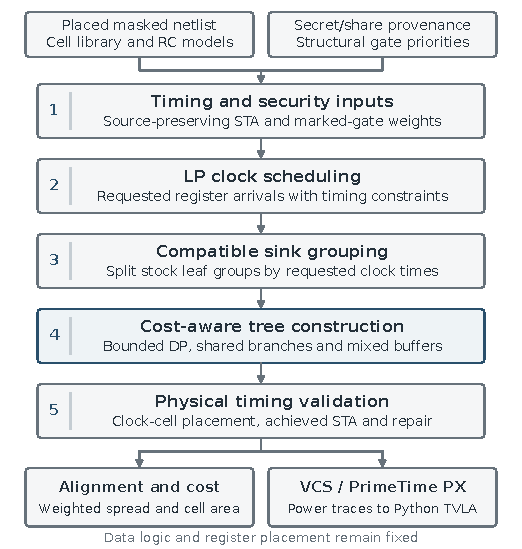
\includegraphics[width=\columnwidth]{figures/flow.pdf}
\caption{Proposed flow. Planning produces requested arrivals; construction and STA determine achieved timing. Power and TVLA are separate downstream measurements.}\label{fig:flow}
\end{figure}

The hierarchy limits the topology space before buffer implementation search. It is not an enumeration of every clock tree. Within that hierarchy, however, a subtree can have several physical implementations. A low-cost leaf chain can load its parent differently from a faster chain, and a shared prefix can change both latency and capacitance. Keeping only the locally fastest or cheapest implementation can remove a choice needed by an ancestor.

\subsection{Bounded bottom-up search}
The constructor retains a frontier of candidate states. Each state represents actual buffer-chain choices and links to selected child states, together with timing statistics, capacitance, estimated energy, buffer count, and depth. At an internal node, candidate child combinations are joined with candidate shared-prefix implementations. The resulting states are evaluated and pruned before being passed upward.

A conceptual recurrence is
\begin{equation}
\mathcal F_v=\operatorname{Prune}_B\{\operatorname{Combine}(p,s_1,s_2)\},
\end{equation}
with $p\in\mathcal P_v$, $s_1\in\mathcal F_{v_1}$, and $s_2\in\mathcal F_{v_2}$. Here $\mathcal P_v$ denotes permitted local implementations, $\mathcal F_v$ the retained subtree states, and $B$ the bound on retained alternatives. This describes bottom-up search on the chosen hierarchy, not an exact global optimization over every physical tree. Quantized latency buckets and a capped frontier bound computation. Retention preserves useful timing alternatives alongside low-cost states so that one type does not eliminate the other prematurely.

The search can be deterministic for fixed inputs and ordering while still exploring multiple alternatives. Determinism describes repeatability, not the absence of search. Approximation arises from the chosen hierarchy, discretized timing representation, finite implementation choices, and restricted frontier. The best retained state therefore need not be the best state in the unrestricted design space. This is why the method is described as bounded approximate DP.

\subsection{Estimated cost and mixed buffer strengths}
The constructor ranks candidate implementations using target-timing error and an energy proxy informed by cell characterization and capacitive loading. This proxy helps compare clock-tree alternatives but is not the measured total power of the complete circuit. The selected construction uses an energy-weight setting of 40, permits BUF\_X1 through BUF\_X16, and specifies BUF\_X4 as the root buffer in the construction invocation.

Mixed strengths remove the need for a strong leaf driver everywhere. A lightly loaded or timing-tolerant branch can use a smaller implementation while a demanding branch retains a stronger driver. This can reduce clock-cell area and switching cost. The tradeoff is that a cheaper choice may change slew or arrival enough to affect setup and hold. Cost-oriented construction therefore remains coupled to timing verification.

\subsection{Calibration, placement, and selective repair}
Earlier measured constructions supply calibration information such as branch slew and common delay corrections. Calibration improves the model for a later construction but does not make requested and achieved arrivals identical. After instantiation, detailed placement, propagated-clock analysis, and placement-based parasitic estimation are performed. Data-cell identity and non-clock connectivity are checked against stock.

The selected final circuit includes nine leaf-driver upsizes to BUF\_X4 following timing analysis. This is selective repair after mixed-strength construction, rather than restoring strong drivers on every leaf. All reported results refer to the repaired circuit. The power campaign therefore evaluates the same physical design whose native weighted-skew improvement is reported.

These stages must be distinguished. The LP provides a schedule; bounded DP provides an implementation under an approximate model; placement and repair produce the measured circuit. Predicted gain cannot replace post-construction gain, and estimated clock energy cannot replace downstream total power. Retaining this separation also helps diagnose whether a disappointing result originates in planning, physical target delivery, or the relationship between the timing surrogate and switching activity.

\section{Experimental Methodology}
\subsection{Circuit and physical conditions}
The experiment compares frozen PRESENT stock with the selected mixed-strength DP circuit. Both use typical Nangate45 models and placement-estimated interconnect parasitics. Register and data-cell placement is unchanged, so the principal changes are in the clock network. No claim of detailed-route extraction, multi-corner signoff, or silicon measurement is made.

Native STA measures the original marked-gate objective, setup and hold slack, electrical checks, and overhead. A separate flow exports the same circuit as a gate-level netlist with simulation delays, parasitics, and constraints. VCS applies input vectors and produces switching activity. PrimeTime checks timing independently, and PrimeTime PX computes time-based modeled power with glitch modeling enabled. Python analyzes aligned power windows; it does not substitute toggle counts for the power tool.

\subsection{Matched stimulus and power collection}
The completed campaign contains four runs: stock and candidate, each under fixed-versus-random (FVR) stimulus and random-versus-random null control. Each run has 1,024 functional transactions, 512 traces per class. The clock period is 2 ns, or 500 MHz. A transaction includes 40 guard cycles and a measured window of 40 cycles, giving an 80 ns trace. Inputs are driven 0.2 ns after the rising edge according to the recorded protocol.

The fixed FVR secret is the all-zero 64-bit value. Fresh independent 64-bit input masking and 368-bit randomness are provided per guard/measurement transaction. Stock and candidate receive matched vectors and identical per-mode window manifests. This controls differences in stimulus and alignment while preserving the distinct physical responses caused by their networks.

Power is requested at 5 ps resolution, giving 16,000 bins per window. All four saved simulation logs report completion of 1,024 functional transactions without reported timing-violation, error, or fatal diagnostics. Printed model warnings are audited separately; the saved load-warning audit finds no actual load extrapolations among the checked warnings. Raw power remains unchanged; documented excluded terminal handling occurs in separate analysis copies outside all measured windows.

\subsection{TVLA and reporting endpoint}
First-order TVLA compares class means at each aligned sample using Welch's statistic~\cite{tvla}:
\begin{equation}
t_j=\frac{\bar x_{0j}-\bar x_{1j}}{\sqrt{s_{0j}^{2}/n_0+s_{1j}^{2}/n_1}}.
\label{eq:welch}
\end{equation}
Here $\bar x_{cj}$ and $s_{cj}^{2}$ are the sample mean and variance for class $c$ at bin $j$, and $n_c$ is its trace count. The campaign reports signed curves, the maximum absolute statistic, and bins exceeding the declared absolute threshold of 4.5. Null controls use the same pipeline. The full 512-per-class endpoint is retained even when exploratory smaller prefixes behave differently.

The test uses aggregate modeled power, not an isolated sensitive-glitch waveform. The separate PX glitching-power report measures an aggregate category without identifying which glitches carry secret information. A lower glitch-power number and a lower FVR peak are therefore distinct observations rather than one validating the other.

\section{PRESENT Results and Analysis}
\subsection{Weighted skew, target tracking, and timing}
Table~\ref{tab:native} summarizes native measurements. Weighted cost decreases from 1454.033 to 1215.255 weighted ns, a 16.42\% reduction. Unweighted mean spread also decreases from 70.172 to 59.403 ps. The latter corroborates the trend but does not replace the weighted objective, which prioritizes gate categories differently.
\begin{table}[!t]
\caption{PRESENT native timing and physical measurements.}\label{tab:native}
\centering\begin{tabular}{lrr}\hline
Metric & Stock & Proposed\\\hline
Weighted cost (weighted ns) & 1454.033 & 1215.255\\
Mean spread (ps) & 70.172 & 59.403\\
Setup slack (ns) & 1.41427 & 1.42323\\
Hold slack (ps) & 10.046 & 18.643\\
Total cell area ($\mu$m$^2$) & 40018.902 & 40063.590\\
Clock-cell area ($\mu$m$^2$) & 701.974 & 804.916\\\hline
\end{tabular}
\end{table}

Improvement is not uniform. Of 5,088 marked gates, 3,055 improve and 987 regress; 2,053 improve by at least 1 ps. There are 428 gates worsening by more than 5 ps, 196 by more than 10 ps, and 28 by more than 20 ps. Maximum regression is 45.256 ps. The result therefore passes the reporting policy that assesses aggregate gain while recording regressions, but not a hard 5 ps per-gate worsening cap. The LP's soft penalty must not be interpreted as a physical bound.

The achieved spread distribution retains a long tail. The median is 28.942 ps; the 90th, 95th, and 99th percentiles are 159.172, 181.771, and 230.731 ps. The worst marked-gate spread is 307.254 ps. Aggregate improvement does not mean all sensitive meetings are tightly aligned. Explicit protection of tail gates could be investigated, but would introduce additional constraints and a different tradeoff.

Requested and achieved clocks differ: RMS target error is 12.452 ps and maximum error is 30.161 ps. Maximum measured clock movement is 71.218 ps, below the configured 80 ps acceptance bound. These values quantify the gap between planning and physical construction and justify reporting measured rather than requested gain.

Native setup and hold slack remain positive and the electrical-pass flag is set. Setup slack improves by approximately 8.96 ps and hold slack by 8.60 ps relative to stock. These are placement-based values, not a worst-case signoff statement across process corners. They establish that the skew improvement is not being reported from a candidate that fails its native timing screen.

\subsection{Physical cost and total power}
The final tree contains 673 clock cells including the recorded dummy-load accounting, with approximately 15,053.993 $\mu$m of clock-pin half-perimeter wirelength. This is a placement proxy, not extracted routed clock-wire length. Total cell area increases by approximately 0.112\%, while clock-cell area increases by 14.66\%. A small whole-design area change can conceal a larger change in the clock subsystem.

Table~\ref{tab:power} gives the power results. FVR measured-window total power increases from 20.8968 to 21.6435 mW: 0.7468 mW or 3.57\%. The selected circuit is a low-overhead skew-improvement point, not a circuit with total power below stock. Mixed-strength construction addresses the cost of delivering targets, but the remaining clock overhead is not fully offset by the observed data-activity changes.
\begin{table}[!t]
\caption{PRESENT power and full-sample TVLA results.}\label{tab:power}
\centering\begin{tabular}{lrr}\hline
Metric & Stock & Proposed\\\hline
FVR window power (mW) & 20.8968 & 21.6435\\
Full-run glitching power ($\mu$W) & 30.050 & 22.920\\
FVR peak $|t|$ & 2.896 & 2.581\\
Null-control peak $|t|$ & 3.014 & 3.056\\
FVR crossing bins & 0 & 0\\
Null crossing bins & 0 & 0\\\hline
\end{tabular}
\end{table}

Full-run aggregate glitching power falls from 30.050 to 22.920 $\mu$W, a 23.73\% reduction. This is consistent with reduced aggregate transient-switching cost in the modeled run, but does not isolate secret-dependent glitch energy. The glitch report averages the full run including guard and initialization activity, whereas total power above averages selected windows. Subtracting the numbers would mix averaging domains and cannot yield a valid non-glitch power estimate.

Fig.~\ref{fig:power} shows mean power over a compact part of the recorded trace. Lower peaks can coexist with a higher average when transitions are redistributed or broadened. Peak height cannot replace integration over the declared window. The numerical average in Table~\ref{tab:power} remains the comparison metric.
\begin{figure}[!t]
\centering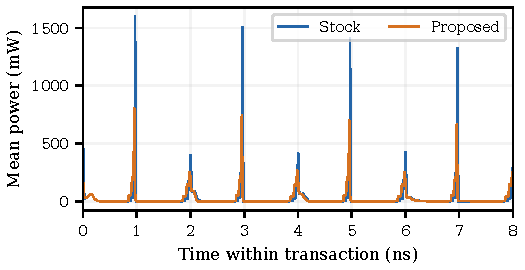
\includegraphics[width=\columnwidth]{figures/power.pdf}
\caption{Class-balanced mean power during the first 8 ns of the 80 ns trace. This crop improves readability; reported average power uses the full window.}\label{fig:power}
\end{figure}

\subsection{Full-sample leakage statistics}
Fig.~\ref{fig:tvla} shows the complete 80 ns FVR and null curves. The candidate's FVR peak absolute statistic decreases from 2.896 to 2.581. Neither crosses 4.5 at 512 traces per class. The null peak changes from 3.014 to 3.056, also without crossing. These observations do not demonstrate elimination of detectable baseline leakage: stock already lacks a full-sample crossing in this campaign.
\begin{figure}[!t]
\centering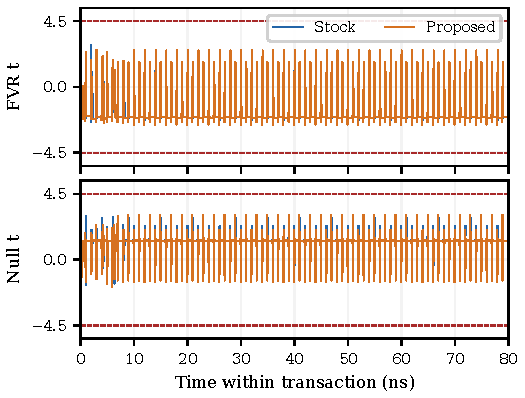
\includegraphics[width=\columnwidth]{figures/tvla.pdf}
\caption{Full-sample PRESENT Welch statistics: FVR above and random/random control below. Dashed lines mark $\pm4.5$; both designs use 512 traces per class.}\label{fig:tvla}
\end{figure}

The sign of $t$ indicates which class has the larger mean; the threshold comparison uses its magnitude. A smaller peak can reflect a smaller mean difference, a larger within-class variance, or both. It is not a calibrated percentage reduction in leakage or an estimate of extra traces needed for key recovery. No attack-success experiment or independent-seed replication is included.

\subsection{Sample-count sensitivity}
Exploratory prefixes show why the endpoint needs context. Table~\ref{tab:prefix} uses the first 128, 256, and 512 traces per class. With 128 per class both FVR curves cross. With 256 per class the candidate still crosses while stock does not. The full endpoint is the declared larger-sample comparison, not evidence that unfavorable smaller-sample results can be discarded.
\begin{table}[!t]
\caption{FVR prefix sensitivity: peak $|t|$ (crossing bins).}\label{tab:prefix}
\centering\begin{tabular}{rrr}\hline
Traces per class & Stock & Proposed\\\hline
128 & 5.283 (198) & 5.316 (45)\\
256 & 4.129 (0) & 4.591 (36)\\
512 & 2.896 (0) & 2.581 (0)\\\hline
\end{tabular}
\end{table}

Null prefixes also cross: peaks are approximately 5.80 at 128 per class and 4.87--4.92 at 256 per class. These are correlated subsets, not independent experiments, and must not be counted as replicated evidence. Their behavior motivates independent seeds and sensitivity checks before interpreting the lower full-sample FVR peak as a reliable security improvement.

\section{Discussion and Limitations}
The results support a specific claim: fixed-placement CTS reduces the original weighted data-skew objective on this PRESENT layer while satisfying the reported native timing checks and limiting total-power overhead to 3.57\%. They also show lower tool-reported aggregate glitching power. They do not establish that 8/4/2 is an optimal leakage weighting, that the tree is globally optimal, or that the statistical trend generalizes to other circuits.

Approximations occur at multiple levels. Conservative marking can overestimate secret dependence. The LP translates frozen windows instead of recomputing nonlinear slew-dependent responses during optimization. Group splitting restricts shared targets. Hierarchy selection and bounded frontiers restrict physical search. Placement parasitics approximate eventual routing. Each can contribute to target error or unfavorable power cost; failure to reach a requested gain need not implicate a single stage.

The source and cost models also optimize different quantities. The LP controls weighted skew, whereas the constructor balances target error against estimated clock energy. Neither directly minimizes measured sensitive-glitch power. A future formulation could couple target selection to a calibrated implementation-cost estimate while retaining the original objective for comparison. It should not change weights and then present the resulting scores as directly equivalent.

Independent seeds would test statistical stability. Matched averaging domains would support a power-component breakdown. Routed parasitics and multiple corners would test physical robustness. Gate-level activity analysis could examine whether timing improvements at marked gates actually explain the reduced glitch category. These are future experiments, not demonstrated properties of the current dataset.

\section{Conclusion}
Source-preserving timing extraction, LP clock planning, compatible grouping, and bounded DP construction reduce weighted data-arrival spread in a masked PRESENT layer. The selected mixed-strength implementation, including nine selective leaf repairs, achieves 16.42\% measured weighted-skew reduction with fixed data placement. Aggregate glitching power falls by 23.73\%, while measured-window total power remains 3.57\% above stock. The FVR peak decreases from 2.896 to 2.581, but endpoint non-crossing, prefix crossings, and absent independent-seed replication limit security interpretation. The contribution is a measured CTS tradeoff between data alignment and implementation cost, with the optimized objective distinguished from downstream leakage observations.

\begin{thebibliography}{00}
\bibitem{present} A. Bogdanov, L. R. Knudsen, G. Leander, C. Paar, A. Poschmann, M. J. B. Robshaw, Y. Seurin, and C. Vikkelsoe, ``PRESENT: An ultra-lightweight block cipher,'' in \emph{CHES}, 2007, pp. 450--466.
\bibitem{glitch} Z. Zhang, S. Nikova, and V. Nikov, ``Glitch-stopping circuits: Hardware secure masking without registers,'' Cryptology ePrint Archive, 2024/891, 2024, doi: 10.1145/3658644.3670335.
\bibitem{sta} The OpenROAD Project, ``OpenSTA,'' source and documentation. \texttt{github.com/\allowbreak The-OpenROAD-Project/\allowbreak OpenSTA}. Accessed Nov. 11, 2026.
\bibitem{cts} The OpenROAD Project, ``Clock tree synthesis,'' documentation. \texttt{openroad.readthedocs.io/\allowbreak en/\allowbreak latest/\allowbreak main/\allowbreak src/\allowbreak cts/\allowbreak README.html}. Accessed Nov. 11, 2026.
\bibitem{scipy} SciPy Developers, ``scipy.optimize.linprog,'' API documentation. \texttt{docs.scipy.org/\allowbreak doc/\allowbreak scipy/\allowbreak reference/\allowbreak generated/\allowbreak scipy.optimize.linprog.html}. Accessed Nov. 11, 2026.
\bibitem{tvla} G. Goodwill, B. Jun, J. Jaffe, and P. Rohatgi, ``A testing methodology for side-channel resistance validation,'' NIST Non-Invasive Attack Testing Workshop, 2011.
\end{thebibliography}
\end{document}
